%%% In this section, you will describe all of the various artifacts that you will generate and maintain during the project life cycle. Describe the purpose of each item below, how the content will be generated, where it will be stored, how often it will be updated, etc. Replace the default text for each section with your own description. Reword this paragraph as appropriate.

\subsection{Major Documentation Deliverables}
%%% intentionally left blank
\subsubsection{Project Charter}
Version 1 of the Project Charter will be delivered on October 4, 2021 with Version 2 being delivered on December 6, 2021 and the final version being delivered on  May 3, 2022. The Project Charter will be reviewed every week during team meetings and will only be updated if four out of five team members agree on the update. The team will review and approve the Project Charter in the meeting that most immediately precedes the Charters due dates.

\subsubsection{System Requirements Specification}
Version 1 of the System Requirements Specification will be delivered on October 25, 2021 with Version 2 being delivered on December 6, 2021 and the final version being delivered on May 3, 2022 . The System Requirements Specification will be reviewed every week during team meetings and will only be updated if four out of five team members agree on the update. The team will review and approve the System Requirements Specification in the meeting that most immediately precedes the System Requirements Specification due dates.

\subsubsection{Architectural Design Specification}
Version 1 of the Architectural Design Specification will be delivered on November 15, 2021 with Version 2 being delivered on December 6, 2021 and the final version being delivered on May 3, 2022 . The Architectural Design Specification will be reviewed every week during team meetings and will only be updated if four out of five team members agree on the update. The team will review and approve the Architectural Design Specification in the meeting that most immediately precedes the Architectural Design Specification due dates.

\subsubsection{Detailed Design Specification}
Version 1 of the Detailed Design Specification will be delivered on February 22, 2022 and the final version being delivered on April 21, 2022. The Detailed Design Specification will be reviewed every week during team meetings and will only be updated if four out of five team members agree on the update. The team will review and approve the Detailed Design Specification in the meeting that most immediately precedes the Detailed Design Specification due dates.

\subsection{Recurring Sprint Items}
\subsubsection{Product Backlog}
Items will be added to the product backlog based on requirements from the customer and will only be done as a group. No members will be permitted to add items without the rest of the teams knowledge and approval. Priority will be given to backlog items based on the customers input. All other items will then be given priority by the team through majority vote of four to one. The teams backlog will be maintained and accessible to all members via Jira. 

\subsubsection{Sprint Planning}
This project will have eight confirmed sprints with the possibility to add any during the winter break. All sprints will be planned by the team on the Fridays immediately preceding the beginning of the sprint. 

\subsubsection{Sprint Goal}
The customer will be given the option to set the team's sprint goal(s). In the case that the customer does not provide any, the sprint goal(s) will set by the team during the sprint planning meeting. These team set goals will be based on the priority of product backlog items and due dates of required documentation.

\subsubsection{Sprint Backlog}
The team's sprint backlog will be set before every sprint. The sprint backlog will be set based on the priority of items on the product backlog as well as estimated person hours needed to complete those items. The team will maintain the sprint backlog along with a scrum board via Jira.

\subsubsection{Task Breakdown}
Items from the sprint backlog will be assigned on Jira on a volunteer basis. This will allow for members to volunteer for items that would provide them an opportunity to learn something new while also creating the ability for team members to take on items they already know how to do when time becomes a bigger factor.

\subsubsection{Sprint Burn Down Charts}
The team manager will be responsible for the sprint burn down chart. The manager will use Jira to populate the burn down chart, but all members will be responsible for updating the progress of their assigned backlog items and logging the hours they put into completing those items. See Figure 1 for an example.

\begin{figure}[h!]
    \centering
    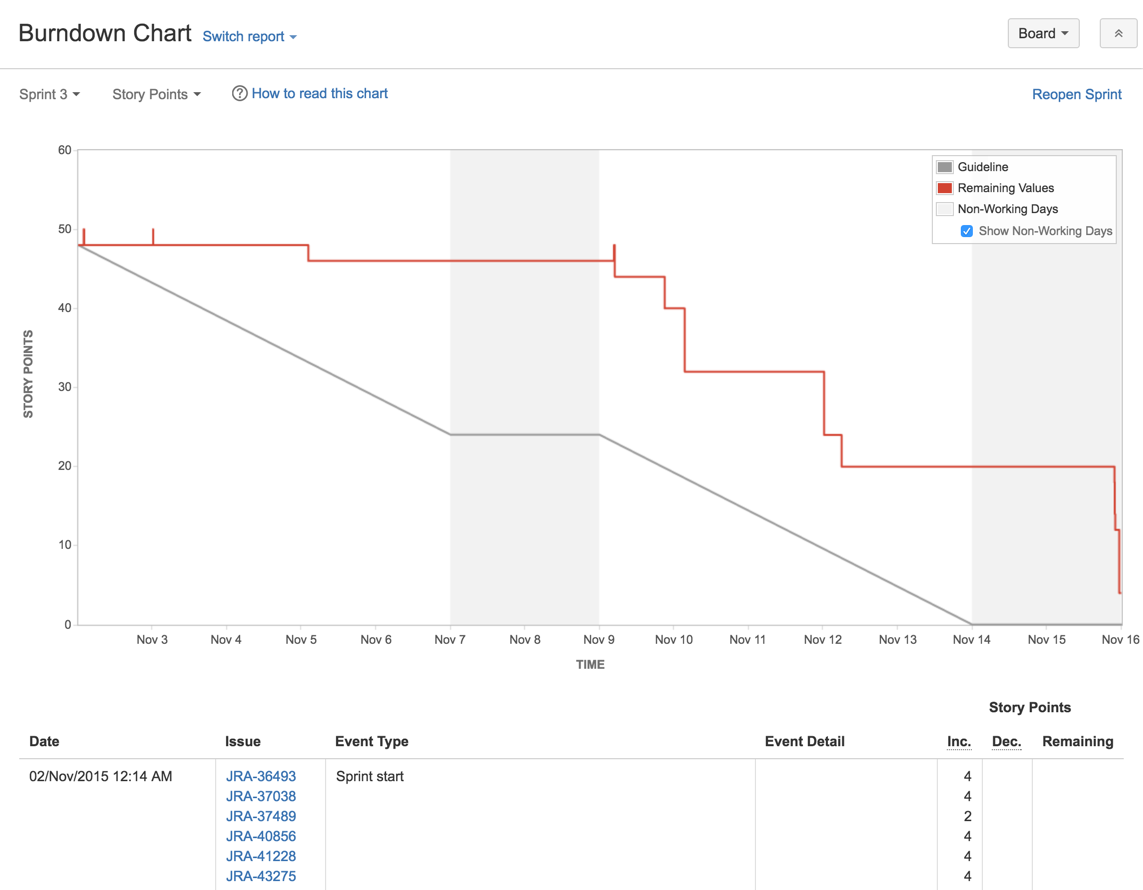
\includegraphics[width=0.5\textwidth]{images/burndown}
    \caption{Example sprint burn down chart}
\end{figure}

\subsubsection{Sprint Retrospective}
The sprint retrospective will be created by all team members during the sprint review session that will take place during the Friday meetings at the end of each sprint. During these sprint review sessions, all team members will discuss the status of each sprint backlog items, the person hours put into them, and the team manager will populate the sprint burn down chart.

\subsubsection{Individual Status Reports}
Individual Status Reports are to be completed by each individual team member immediately following the end of sprints. Team members will use the sprint goal, sprint backlog, and sprint burn down chart that is agreed upon by the team. Team members will also use the sprint review session to help in the assessment of other team members. The sprint review session can also be used to create individual goals for the upcoming sprint. 

\subsubsection{Engineering Notebooks}
Each team member will be solely responsible for filling out their engineering notebook. Due to the setting of this project, all team members will disregard the witness signature for the engineering notebook.

\subsection{Closeout Materials}
\subsubsection{System Prototype}
The aim of this project is to meet all of the customer's requirements in the final system prototype. The final system prototype will first be demonstrated to the customer during the Prototype Acceptance Test. The final demonstration will take place on April 21, 2022.

\subsubsection{Project Poster}
The project poster will be delivered on April 21, 2022 during the final demonstration. The project poster will contain the system requirements, architectural design and design specifications and be 24" x 36". 

\subsubsection{Web Page}
The project web page will be hosted on the University's senior design project repository. The web page will be accessible to the public and be delivered on April 21, 2022. The web page will contain; the team name, the product name, the timeline that the team worked on the project, all team member's names, an abstract, background, project requirements, system overview, demo video, future plans and improvements for the project, and links to all documents and source code. 

\subsubsection{Demo Video}
The demo video will walk viewers through the entire user interface while also showing all the requirements that were met. The demo video should be under five minutes.

\subsubsection{Source Code}
All source code will be maintained in a private GitHub repository that will be accessible by all team members. Due to our customer's experience and knowledge of this project, they will have access to all source code upon request. This project will not be open sourced to the general public.

\subsubsection{Source Code Documentation}
Each team member will be responsible for properly documenting all code. Formal documentation will be generated with Doxygen and will be provided in LATEX format.

\subsubsection{Installation Scripts}
In the case that this project will be created for use on a mobile device (Android or iOS) the project will be added to the corresponding application stores which will allow for the customer, and any other user, to have access to the project. In the case that this project is to be a desktop application, installation scripts will be provided to allow for the automatic installation for the customer.

\subsubsection{User Manual}
A short, easy to read user manual will be provided in the application that will be accessible to all users. A more detailed user manual will provided digitally to the customer in PDF format.
